\documentclass[12pt]{article}
\usepackage[russian]{babel}
\usepackage[utf8]{inputenc}
\inputencoding{utf8}
\usepackage{geometry}\geometry{a4paper, margin=2cm}
\usepackage[numbers,sort&compress,square]{natbib}
\usepackage{hyperref,xcolor}
\usepackage{graphicx,caption,subcaption}
\usepackage{indentfirst,amsmath,amssymb,textcomp}
\usepackage{url}
\sloppy
\title{Численное решение уравнения Пуассона. Распределение поля в конденсаторе.}
\author{}
\date{}

\renewcommand{\vec}[1]{\textbf{#1}}
\newcommand{\task}[2]{\vspace{6pt}
\textbf{Задание #1}. #2 \vspace{6pt}}

\begin{document}
\maketitle

\section*{Конечно-разностная схема решения уравнения Пуассона}
Распределение потенциала электрического поля $U(\vec{r})$ в пространстве при наличии статической плотности зарядов $\rho(\vec{r})$ подчиняется уравнению Пуассона:
%
\begin{equation}
\triangle U(\vec{r})=-4\pi\rho(\vec{r}),
\end{equation}
%
которое совпадает с уравнением Лапласа в случае $\rho(\vec{r})=0$. Это уравнение в частных производных \textit{эллиптического типа}. Если в качестве граничных условий использовано условие Дирихле, то есть задано значение $U$ на границе рассматриваемой области, то решение существует и единственно. В ограниченном количестве случаев можно найти аналитическое решение этого уравнения. Например, в прямоугольной области, на одной границе которой задано конечное значение потенциала, а на остальных он равен нулю, как показано на Рис. \ref{fig:simple}. Решение будет представлено в виде суммы бесконечного ряда Фурье, что не очень удобно с практической точки зрения. Если, например, необходимо построить решение $U(x,y)$, можно учесть лишь конечное количество членов ряда, а так как ряд сходится очень медленно, то количество членов должно быть весьма большим.

\begin{figure}
\begin{minipage}{0.49\linewidth}
\begin{center}
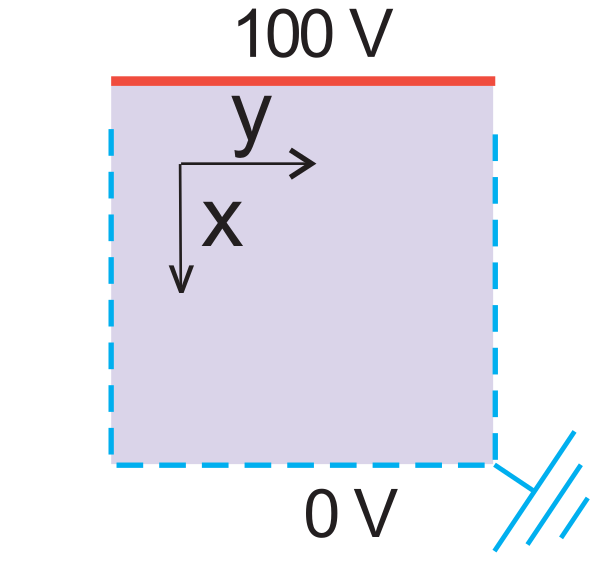
\includegraphics[width=0.9\linewidth]{./figs/01.png}\\
а)
\end{center}
\end{minipage}
\begin{minipage}{0.49\linewidth}
\begin{center}
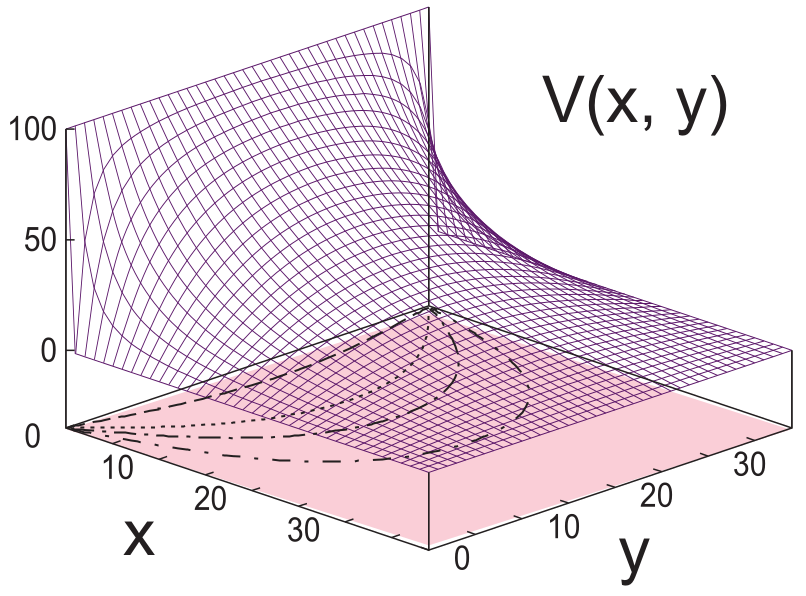
\includegraphics[width=1.1\linewidth]{./figs/02.png}\\
б)
\end{center}
\end{minipage}
\caption{a) На границе, обозначенной красным, задан потенциал, например, 100 V. Можно найти решение во всей области, обозначенной серым цветом; б) распределение потенциала $U(x,y)$.}
\label{fig:simple}
\end{figure}

\begin{figure}
\begin{center}
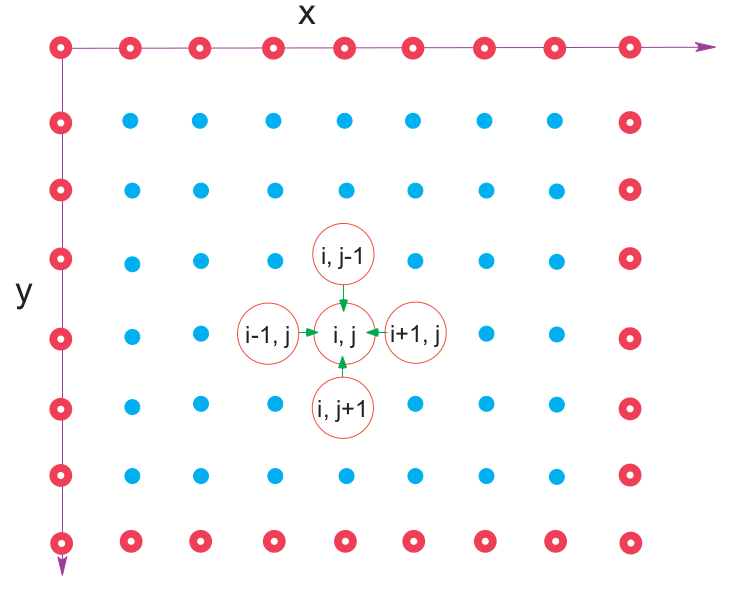
\includegraphics[width=0.5\linewidth]{./figs/03.png}
\end{center}
\caption{Алгоритм решения уравнения Пуассона на решётке.}
\label{fig:algorithm}
\end{figure}

Для численного решения уравнения Пуассона можно использовать \textit{конечно-разностную схему}. Для простоты рассмотрим двухмерную квадратную область. Удобно использовать прямоугольную систему координат, в которой уравнение имеет вид:
%
\begin{equation} 
\frac{\partial^2 U(x,y)}{\partial x^2}+\frac{\partial^2 U(x,y)}{\partial y^2}=-4\pi\rho(x,y).
\label{eq:Poisson}
\end{equation}
%
Вторую производную, например, по координате $x$ можно приближённо представить как
%
\begin{equation}
\frac{\partial^2 U}{\partial x^2}\approx \frac{U(x+\Delta x,y)+U(x-\Delta x,y)-2U(x,y)}{(\Delta x)^2},
\label{eq:derivative}
\end{equation} 
%
и аналогично по $y$. Разобьём область с помощью равномерной решётки $N\times N$ с шагом $\Delta$, как показано на Рис. \ref{fig:algorithm}, так, что $(x,y)=(i,j)\Delta$, где $i,j=\overline{0,N-1}$ (считаем, что точка отсчёта --- $(0,0)$). Можно вычислить производную в каждом узле решётки $(i,j)$ по формуле \eqref{eq:derivative} и переписать приближённое уравнение в следующем виде:
%
\begin{equation}
U_{i+1,j}+U_{i-1,j}+U_{i,j+1}+U_{i,j-1}-4U_{i,j}=-4\pi\rho_{i,j}\Delta^2,
\end{equation}
%
где $U_{i,j}=U(i\Delta,j\Delta)$, $\rho_{i,j}=\rho(i\Delta,j\Delta)$. Это выражение можно рассматривать как уравнение на матрицу $U_{i,j}$, однако решать его напрямую крайне неэффективно из-за большого размера матрицы. Конечно-разностная схема заключается в итеративном решении матричного уравнения 
%
\begin{equation}
U_{i,j}=\frac{1}{4}\left[U_{i+1,j}+U_{i-1,j}+U_{i,j+1}+U_{i,j-1}\right]+\pi\rho_{i,j}\Delta^2.
\end{equation}
%
Выбирается некоторое пробное начальное распределение $U^0_{i,j}$ (вообще говоря, любое), подставляется в правую часть этого уравнения, после чего вычисляется новое значение матрицы $U^\text{new}_{i,j}$ (см. также Рис. \ref{fig:algorithm}). Затем матрица $U^\text{new}_{i,j}$ снова подставляется в правую часть уравнения и операция повторяется. Итерации необходимо проводить до тех пор, пока результат не сойдётся к решению (также говорят \textit{релаксирует}). Отметим, что в точках по краям области $U$ задано граничное условие, то есть значения $U_{0,j}$, $U_{N-1,j}$, $U_{i,0}$, $U_{i,N-1}$ фиксированы.

На данном этапе существует два чрезвычайно важных вопроса: 1) сходится ли схема к истинному решению, и 2) если сходится, то как быстро? В большом количестве учебников по численным методам можно найти аккуратное доказательство устойчивой сходимости к точному решению рассмотренной схемы для эллиптического уравнения с граничным условием Дирихле, поэтому первый вопрос будем считать закрытым. Однако стоит обратить внимание, что это далеко не всегда так в случае уравнений другого типа или в случае нелинейных уравнений, поэтому при решении задач разностными методами стоит внимательно подойти вопросу устойчивости и сходимости, иначе результат бездумного применения численной схемы может не иметь ничего общего с истинным решением уравнения!

Скорость сходимости метода может быть различной в зависимости от использованного подхода:
\begin{itemize}
\item \textbf{Метод Якоби} --- прямая реализация описанного выше метода. При каждом вычислении $U^\text{new}_{i,j}$ матрица на предыдущем шаге $U^\text{old}_{i,j}$ неизменна, обход элементов сетки происходит последовательно по $i$ и $j$ согласно Рис. \ref{fig:algorithm} (хотя данное условие является необязательным, оно вводится для того, чтобы была понятна работа следующего метода). Данный метод хорош тем, что позволяет записать одну целую итерацию по $U$ с помощью матричных операций Numpy без использования циклов.

\item \textbf{Метод Гаусса-Зейделя} --- при вычислении $U^\text{new}_{i,j}$ в каждой точке матрица из правой части уравнения сразу обновляется. Это приводит к тому, что элементы $U_{i-1,j}=U^\text{new}_{i-1,j}$ и $U_{i,j-1}=U^\text{new}_{i,j-1}$, но при этом $U_{i+1,j}=U^\text{old}_{i+1,j}$ и $U_{i,j+1}=U^\text{old}_{i,j+1}$. Данный метод хорош тем, что ускоряет сходимость к решению и позволяет экономить память, поскольку не нужно одновременно хранить новую и предыдущую $U_{i,j}$, достаточно только одной матрицы.

\item \textbf{Метод релаксации} или successive over-relaxation. Итерацию можно представить в виде
%
\begin{equation}
U^\text{new}_{i,j}=U^\text{old}_{i,j}+r_{i,j},
\end{equation}
%
где $r$ вычисляется согласно методу Якоби или Гаусса-Зейделя. Для ускорения сходимости предлагается ввести коэффициент $\omega$ так, что
%
\begin{equation}
U^\text{new}_{i,j}=U^\text{old}_{i,j}+\omega r_{i,j}.
\end{equation}
%
При $\omega=1$ схема сходится к решению со скоростью метода, выбранного для вычисления $r$, при $0<\omega<1$ происходит замедление, а выбор $\omega>1$ может дать ускорение сходимости. Однако такое ускорение не всегда даёт положительный эффект, при $\omega>2$ скорее всего возникнет неустойчивость, и сходимости к решению не будет. Параметр $\omega$ может зависеть от размера матрицы, начальных условий и распределения зарядов.
\end{itemize}

\textbf{Критерий сходимости}. По мере прохождения итераций пробные значения матрицы $U_{i,j}$ приближаются к решению уравнения, и в каждой итерации изменения становятся всё меньше. Для оценки того, достигнуто решение или нет, в самом простом варианте <<в лоб>> можно визуально оценивать изменения в графике распределения $U$ и принять решение на какой-то итерации, когда изменения покажутся достаточно малыми, но такой метод явно далёк от научного. По этой причине введём меру
%
\begin{equation}
||U||=|\textrm{tr}(U)|.
\end{equation}
%
Будем считать, что решение достигнуто, если отклонение меры мало $\text{abs}\left(||U^\text{new}||-||U^\text{old}||\right)<\varepsilon$ (или $\text{abs}\left(||U^\text{new}||-||U^\text{old}||\right)/||U^\text{old}||<\varepsilon$), где $\varepsilon$ --- некоторое маленькое число.


\section*{Задание}
\task{1}{\textit{(5 баллов)} Найдите аналитическое решение уравнения Лапласа в области, указанной на Рис. \ref{fig:simple}a). Постройте график распределения потенциала $U(x,y)$ аналогичный Рис. \ref{fig:simple}б) или в виде карты, постройте эквипотенциальные поверхности. При этом учтите, что гиперболические функции, которые должны появиться в решении, растут экспоненциально быстро, поэтому упростите аналитическое выражение так, чтобы избежать переполнения данных (слишком больших чисел). Сколько членов ряда нужно учесть в сумме, чтобы устранить осцилляции на границе?

Примеры построения трёхмерных графиков: \url{https://matplotlib.org/mpl_toolkits/mplot3d/tutorial.html}

Пример построения карт: \url{https://matplotlib.org/gallery/images_contours_and_fields/pcolormesh_levels.html}

Цветовые схемы в Matplotlib: \url{https://matplotlib.org/examples/color/colormaps_reference.html}

Построение эквипотенциальных линий: \url{https://matplotlib.org/examples/pylab_examples/contour_demo.html}.
}

\task{2}{\textit{(5 баллов)} Напишите простейший вариант программы для нахождения потенциала $U(x,y)$ методом Якоби для граничных условий, обозначенных на Рис. \ref{fig:simple} (т.е. решение уравнение Лапласа). Для простоты можно взять сетку $100\times 100$ и  фиксированное число итерации порядка 100-1000. Реализуйте метод Якоби через матричные операции Numpy так, чтобы не использовать циклы в явном виде при выполнении одной итерации.

Программа должна содержать базовый класс --- <<решатель>> уравнения Пуассона, который позволяет задать размер сетки, шаг и число итераций и имеет следующие методы:
\begin{itemize}
\item Метод, вычисляющий состояние матрицы через заданное количество итераций по начальному значению матрицы $U$.
\item Построитель графика распределения $U$ в трёхмерном виде или в виде карты, а также эквипотенциальные линии.
\item Метод \texttt{run}, в котором организовано вычисление потенциала и построение графика. Вызов метода \texttt{run} можно, например, вставить в \texttt{\_\_init\_\_}.
\end{itemize}

Постройте распределение потенциала $U$ в промежуточных состояниях и в конечном состоянии, чтобы увидеть, как пробный потенциал сходится к решению. 

Сравните решение с точным из задания 1.

\textit{Примечание}: так как программа может работать долго, если сетка достаточно мелкая, имеет смысл сохранять изображение на диск функцией Matplotlib \texttt{savefig}. В качестве альтернативы можно сохранять матрицы в сыром виде (текстовые файлы (\texttt{numpy.savetxt}) или бинарные (\texttt{numpy.savez})) и реализовать отдельный построитель графиков, который считывает эти файлы функциями Numpy и позволяет строить распределения. Данный метод является наиболее оптимальным в практических задачах.
}

\task{3}{\textit{(5 баллов)} Усовершенствуйте программу:
\begin{itemize}
\item Реализуйте проверку сходимости по норме.
\item Реализуйте метод Гаусса-Зейделя в качестве отдельного метода класса. Сделайте возможность выбора используемого метода для нахождения потенциала при создании объекта. Например, это можно сделать с помощью ключевых параметров, так что вызов мог бы выглядеть так: \texttt{SolvePoisson(<some params>, method='Jacobi')} или \texttt{SolvePoisson(<some params>, method='Gauss-Seidel')}, и в зависимости от значения \texttt{method} использовался бы метод Якоби или Гаусса-Зейделя.
\item Реализуйте метод релаксации.
\end{itemize}

Протестируйте все три метода на примере из задания 2. Исследуйте метод релаксаций. При каком значении параметра ускорения решение становится неустойчивым? Постройте сравнительные графики для зависимости числа итераций, за которое начальный потенциал сходится к решению, и зависимости скорости исполнения программы от длины сетки по одной стороне $N$.
}

\begin{figure}
\begin{minipage}{0.49\linewidth}
\begin{center}
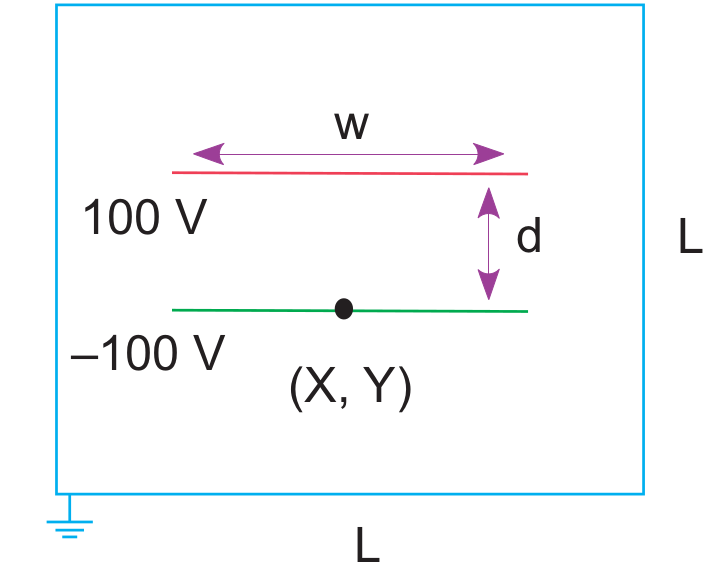
\includegraphics[width=0.9\linewidth]{./figs/04.png}\\
а)
\end{center}
\end{minipage}
\begin{minipage}{0.49\linewidth}
\begin{center}
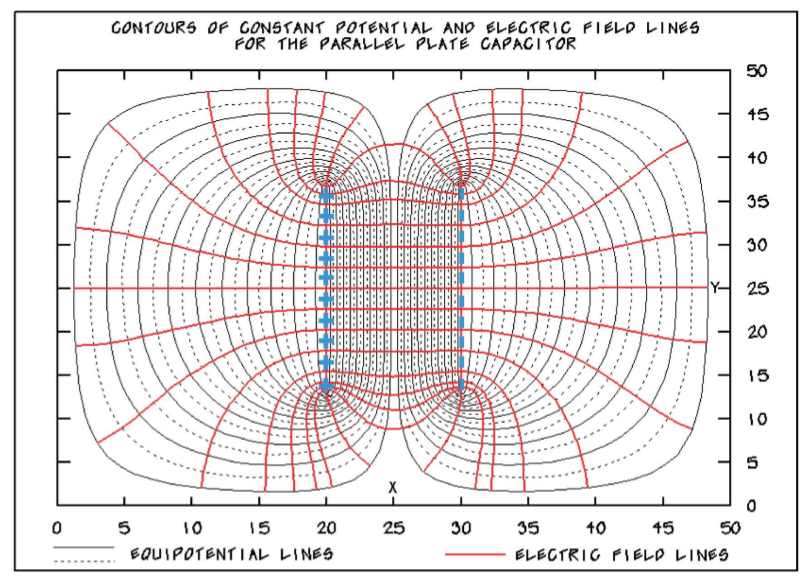
\includegraphics[width=\linewidth]{./figs/05.png}\\
б)
\end{center}
\end{minipage}
\caption{а) Модель конденсатора. б) Эквипотенциальные поверхности и распределение электрического поля в конденсаторе.}
\label{fig:capacitor}
\end{figure}

\task{4}{\textbf{Распределение поля в конденсаторе} \textit{(9 баллов)}. 
\begin{itemize}
\item Простейшая модель конденсатора. Изменим граничное условие на Рис. \ref{fig:simple}а). Пусть две противоположные границы обладают потенциалами 100 V и -100 V. Постройте распределение потенциала.

\item Добавьте метод, который позволяет задавать начальное распределение плотности зарядов. Это может быть функция, чтение из файла с матрицей значений распределения заряда, или считывание изображения (см. библиотеку \url{https://pypi.python.org/pypi/imageio}. В последнем случае можно использовать 2 отдельных файла для описания распределения положительных и отрицательных зарядов в чёрно-белых тонах.

\item Задайте 2 тонких провода с равномерной плотностью заряда $\rho$ и $-\rho$, причем пусть провода находятся внутри области, на границе которой потенциал равен нулю, как показано на Рис. \ref{fig:capacitor}а). Решите уравнение Пуассона. Постройте распределение потенциала и эквипотенциальные линии. Постройте линии электрического поля $\mathbf{E}$, для этого используйте формулы численного дифференцирования потенциала $U$, например, для проекции $E_x$:
%
\begin{equation}
E_{x\,i,j} \approx \frac{U_{i+1,j}-U_{i-1,j}}{2\Delta}.
\end{equation}

\item Придумайте способ задания более сложных областей, внутри которых можно решать уравнение Пуассона или Лапласа. Пусть обкладки конденсатора теперь имеют конечную толщину $\geq 2\Delta$, но при этом фиксированное значение потенциала $\pm 100$ V. Решите уравнение Лапласа во всей области, постройте распределение потенциала и эквипотенциальные поверхности.

Уравнение Пуассона можно использовать для нахождения распределения заряда по заданному потенциалу. Найдите распределение заряда на границе конденсатора с обкладками конечной толщины и постройте его.
\end{itemize}

}

\end{document}
